% \documentclass[handout]{beamer} % Suppress the pauses to print as handout
\documentclass[aspectratio=169, 11pt]{beamer}
% \documentclass[11pt]{beamer} % Comment the line above and use this line for 4:3 aspect ratio screens
\usepackage{advdate}
\usepackage{amsmath}
\usepackage{amsthm}
\usepackage{amsfonts}
\usepackage{amssymb}
\usepackage{array}
\usepackage{color}
\usepackage{helvet}
\usepackage{hyperref}
\usepackage{mathpazo}
\usepackage{multirow}

\usetheme{CambridgeUS}
\usecolortheme{dolphin}
\usefonttheme[onlymath]{serif}

% Define colors considering color blindness
% Use MATLAB default color palette
\definecolor{blue}{rgb}{0, 0.447, 0.741}
\definecolor{red}{rgb}{0.85, 0.325, 0.098}
\definecolor{yellow}{rgb}{0.929, 0.694, 0.125}
\definecolor{purple}{rgb}{0.494, 0.184, 0.556}
\definecolor{green}{rgb}{0.466, 0.674, 0.188}
\definecolor{cyan}{rgb}{0.301, 0.745, 0.933}
\definecolor{magenta}{rgb}{0.635, 0.078, 0.184}
\definecolor{amber}{rgb}{1.0, 0.75, 0.0}

% Self-defined background and frametitle colors
\definecolor{MyBackground}{RGB}{255, 255, 230}
% Uncomment the following line for plain white background
% \definecolor{MyBackground}{RGB}{255, 255, 255}
\setbeamercolor{background canvas}{bg=MyBackground!40}
\setbeamercolor{frametitle}{bg=MyBackground!80}
% Customize word colors
\setbeamercolor{frametitle}{fg=blue}
\setbeamercolor{title}{fg=blue}
\setbeamercolor{itemize item}{fg=blue}
\setbeamercolor{itemize subitem}{fg=blue}
\setbeamercolor{enumerate item}{fg=blue}
\setbeamercolor{enumerate subitem}{fg=blue}
\setbeamercolor{button}{bg=MyBackground,fg=blue}

% Page number on the bottom
\setbeamertemplate{footline}[frame number]
\setbeamerfont{footline}{size=\fontsize{10}{12}\selectfont}
\setbeamercolor{page number in head/foot}{fg=blue}
% No navigation symbols
\setbeamertemplate{navigation symbols}{}
% No headlines
\setbeamertemplate{headline}{}
% Appendix slides don't count
\newcommand{\backupbegin}{
   \newcounter{framenumberappendix}
   \setcounter{framenumberappendix}{\value{framenumber}}
}
\newcommand{\backupend}{
   \addtocounter{framenumberappendix}{-\value{framenumber}}
   \addtocounter{framenumber}{\value{framenumberappendix}}
}
% Add section title at the beginning of each part
\AtBeginSection[]{
  \begin{frame}[noframenumbering, plain]
  \vfill
  \centering
    \begin{beamercolorbox}[sep=8pt, center, shadow=true, rounded=true]{title}
      \usebeamerfont{frametitle}\insertsectionhead\par%
    \end{beamercolorbox}
  \vfill
  \end{frame}
}

% New theorem environments
\newtheorem{thm}{Theorem}
\newtheorem{lem}[thm]{Lemma}
\newtheorem{prop}[thm]{Proposition}

\beamersetuncovermixins{\opaqueness<1>{25}}{\opaqueness<2->{15}}

% Set pause options to be invisible instead of transparent
\setbeamercovered{invisible}

\begin{document}
\title{Lecture 3 \\ Global Approximation Methods}
\author[Wu]{Peifan Wu}
\date{UBC}

\begin{frame}
\titlepage
\end{frame}

\begin{frame}
\frametitle{Global Function Approximation}
  \begin{itemize}
    \item[--] \textcolor{red}{Global Function}: function interpolation over the entire domain
    \bigskip
    \item[--] Types of interpolations:
    \begin{itemize}
      \medskip
      \item[--] \textcolor{blue}{Spectral methods} -- orthogonal polynomials (e.g. Chebyshev, Lagrange, etc) that use \textcolor{red}{global basis}
      \medskip
      \item[--] \textcolor{blue}{Finite element methods} -- splines (e.g. B-splines, cubic splines, Schumaker splines) that use \textcolor{red}{local basis}
    \end{itemize}
    \bigskip
    \item[--] To approximate a known function $f\left(x\right)$ by a linear combination of \textcolor{red}{basis functions} $\phi$
    \[
      f\left(x\right)\equiv\sum_{j=0}^{n}w_{j}\phi_{j}\left(x\right)
    \]
    \begin{itemize}
      \item[--] Basis functions: linearly independent functions that span the family of functions chosen for the interpolation
      \medskip
      \item[--] In general we are interested in the space of $\mathcal{C}^{0}$ and $\mathcal{C}^{1}$ functions
    \end{itemize}
  \end{itemize}
\end{frame}

\begin{frame}
\frametitle{Interpolation}
  \begin{itemize}
    \item[--] The problem boils down to determining the weights $w_{i}$
    \item[--] Several choices:
    \begin{itemize}
      \item[--] \textcolor{red}{Collocation}: use the same number of interpolant nodes as the number of basis functions. $w$ comes from the solution to $\Phi w=y$
      \item[--] If we have more interpolation nodes than basis functions, then we have a "curve fitting" problem. One way is to minimize SSR by applying \textcolor{red}{Least Square},
      \[
        w=\left(\Phi'\Phi\right)^{-1}\Phi'y
      \]
      \item[--] Or apply \textcolor{red}{Galerkin method}: define residuals
      \[
        r(x)=f(x)-\sum_{j=0}^{n}w_{j}\phi_{j}\left(x\right)
      \]
      and solve the equations
      \[
        \int_{a}^{b}r\left(x\right)\phi_{j}\left(x\right)\mathrm{d}x=0,j=0,1,\ldots,n
      \]
    \end{itemize}
    \bigskip
    \item[--] We apply collocation method for the following exercises
  \end{itemize}
\end{frame}

\begin{frame}
\frametitle{Spectral Methods}
  \begin{itemize}
    \item[--] We use polynomial basis
    \bigskip
    \item[--] Why polynomials? \textcolor{red}{Weierstrass Theorem}: if $\mathcal{C}\left[a,b\right]$ is the set of all continuous function on $\left[a,b\right]$ then for all $f\in\mathcal{C}\left[a,b\right]$ and $\epsilon>0$ there exists a polynomial $q$ for which
    \[
      \sup_{x\in\left[a,b\right]}\left|f\left(x\right)-q\left(x\right)\right|<\epsilon
    \]
    \bigskip
    \item[--] Polynomials can approximate any continuous function over a compact domain arbitrarily well
  \end{itemize}
\end{frame}

\begin{frame}
\frametitle{Monomial Basis}
  \begin{itemize}
    \item[--] The most naive procedure: use monomials as basis functions
    \[
      \phi_{j}\left(x\right)=x^{j},j=0,1,\ldots,n
    \]
    with interpolating polynomials of the form
    \[
      \bar{f}\left(x\right)\equiv p_{n}\left(x\right)=w_{0}+w_{1}x+w_{2}x^{2}+\ldots+w_{n}x^{n}
    \]
    \item[--] Use a linear system of $n+1$ equations to solve $w_{i}$
    \[
      \left[\begin{array}{cccc}
      1 & x_{0} & \cdots & x_{0}^{n}\\
      1 & x_{1} & \cdots & x_{1}^{n}\\
      \vdots & \vdots & \ddots & \vdots\\
      1 & x_{n} & \cdots & x_{n}^{n}
      \end{array}\right]\left[\begin{array}{c}
      w_{0}\\
      w_{1}\\
      \vdots\\
      w_{n}
      \end{array}\right]=\left[\begin{array}{c}
      y_{0}\\
      y_{1}\\
      \vdots\\
      y_{n}
      \end{array}\right]
    \]
  \end{itemize}
\end{frame}

\begin{frame}
\frametitle{Monomials in $\left[0,1\right]$}
  \begin{figure}
    \centering
    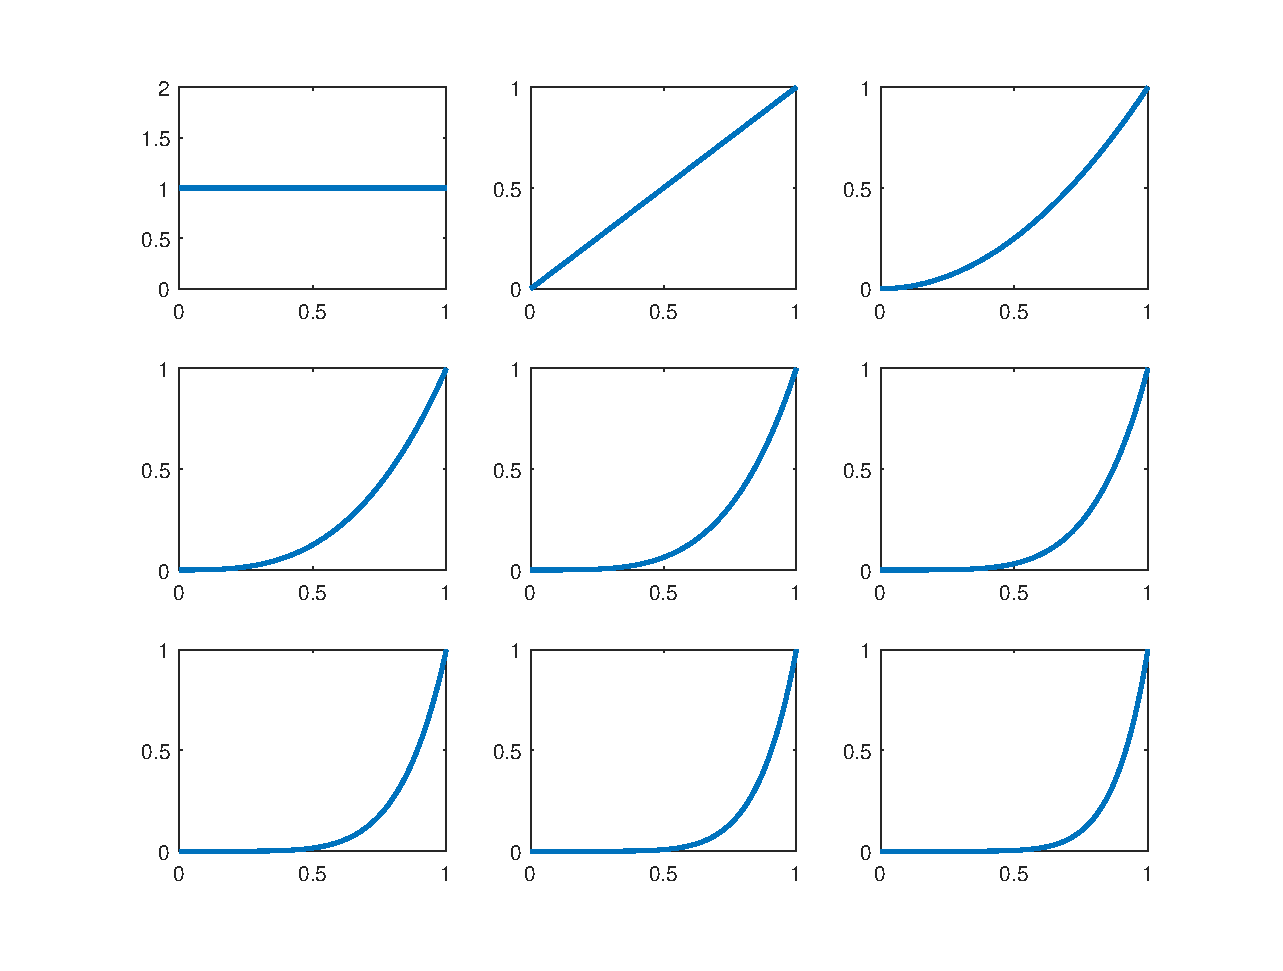
\includegraphics[width = 4in]{monomial.eps}
  \end{figure}
\end{frame}

\begin{frame}
\frametitle{Chebyshev Polynomials}
  \begin{itemize}
    \item[--] Chebyshev polynomials are trigonometric and can be constructed recursively,
    \begin{align*}
      T_{0}\left(x\right) & =1\\
      T_{1}\left(x\right) & =x\\
      T_{k+1}\left(x\right) & =2xT_{k}\left(x\right)-T_{k-1}\left(x\right)
    \end{align*}
    \bigskip
    \item[--] $T_{n}\left(x\right)$ has $n$ distinct roots in $\left[-1, 1\right]$ with expression
    \[
      x_{k}=\cos\left(\frac{2k-1}{2n}\pi\right),k=1,\ldots,n
    \]
    \bigskip
    \item[--] The interpolation nodes that minimize the error of Chebyshev interpolation are the zeros of the Chebyshev polynomials
  \end{itemize}
\end{frame}

\begin{frame}
\frametitle{Chebyshev Basis Functions in $\left[0,1\right]$}
  \begin{figure}
    \centering
    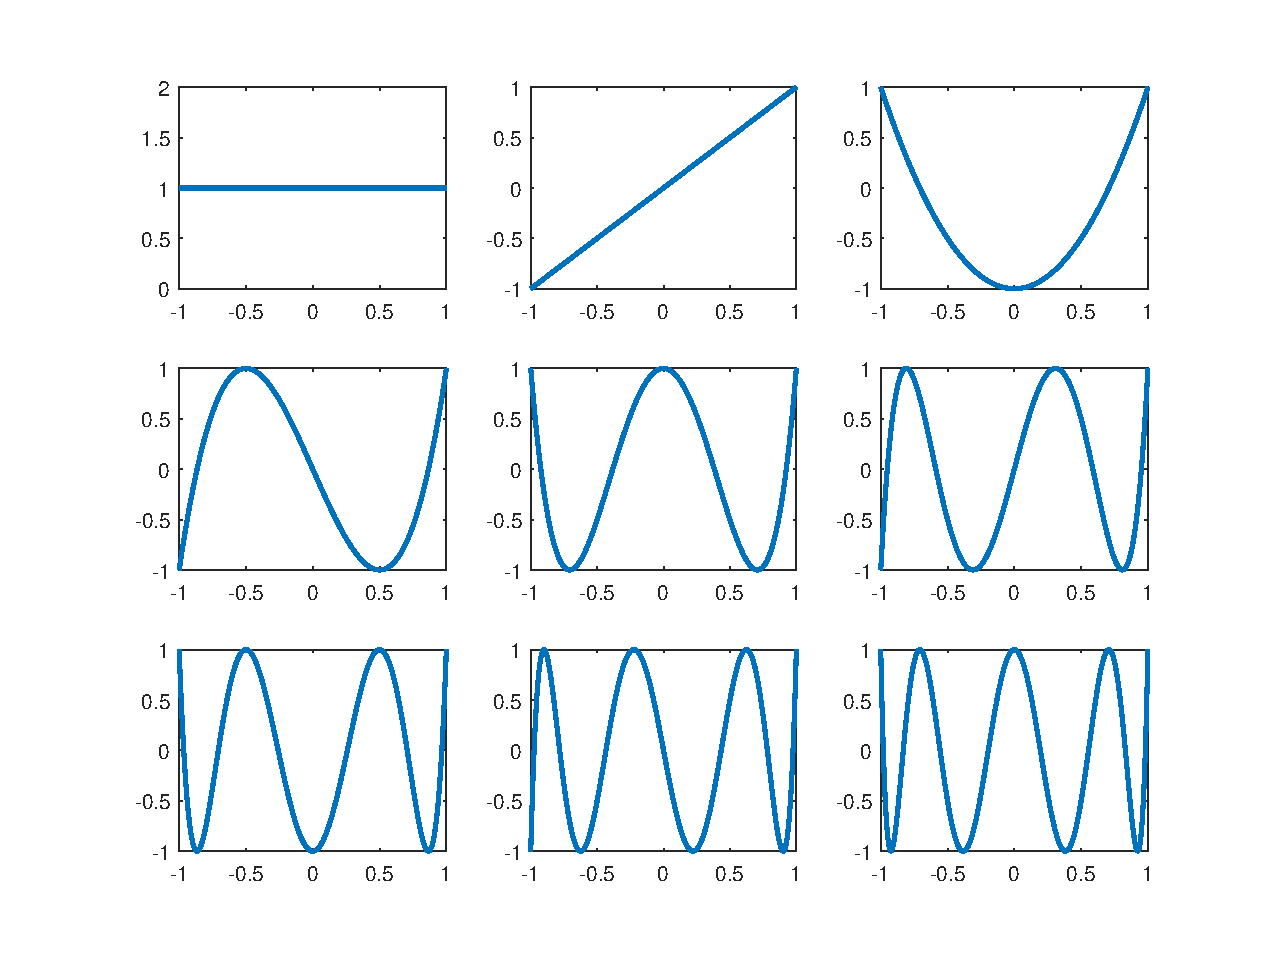
\includegraphics[width = 4in]{chebyshev.eps}
  \end{figure}
\end{frame}

\begin{frame}
\frametitle{Interpolation using Chebyshev Polynomials}
  \begin{itemize}
    \item[--] Choose $x_{i}$ to be the roots of $T_{n}$
    \bigskip
    \item[--] The vector of $w_{i}$ can be obtained as
    \[
      \left[\begin{array}{cccc}
      T_{0}\left(x_{0}\right) & T_{1}\left(x_{0}\right) & \cdots & T_{n}\left(x_{0}\right)\\
      T_{0}\left(x_{1}\right) & T_{1}\left(x_{1}\right) & \cdots & T_{n}\left(x_{1}\right)\\
      \vdots & \vdots & \ddots & \vdots\\
      T_{0}\left(x_{n}\right) & T_{1}\left(x_{n}\right) & \cdots & T_{n}\left(x_{n}\right)
      \end{array}\right]\left[\begin{array}{c}
      w_{0}\\
      w_{1}\\
      \vdots\\
      w_{n}
      \end{array}\right]=\left[\begin{array}{c}
      y_{0}\\
      y_{1}\\
      \vdots\\
      y_{n}
      \end{array}\right]
    \]
    \bigskip
    \item[--] Finally the polynomial approximation of $f$ is
    \[
      \bar{f}\left(x\right)=\sum_{j=0}^{n}w_{j}T_{j}\left(x\right)
    \]
  \end{itemize}
\end{frame}

\begin{frame}
\frametitle{Linear B-splines}
  \begin{itemize}
    \item[--] $B^{1}$ splines implement piecewise linear interpolation
    \[
      B_{k}^{1}\left(x\right)=\begin{cases}
      \frac{x-x_{k-1}}{x_{k}-x_{k-1}} & \text{if }x_{k-1}\leqslant x<x_{k}\\
      \frac{x_{k+1}-x}{x_{k+1}-x_{k}} & \text{if }x_{k}\leqslant x<x_{k+1}\\
      0 & \text{elsewhere}
      \end{cases}
    \]
    it looks like "tent-functions" with peak at $x_{k}$ equal to $1$
    \bigskip
    \item[--] Then the interplant is
    \[
      \bar{f}\left(x\right)=\sum_{k=0}^{n}f\left(x_{k}\right)B_{k}^{1}\left(x\right)
    \]
    \bigskip
    \item[--] Essentially, for $x_{k}<x<x_{k+1}$,
    \[
      \bar{f}\left(x\right)=f\left(x_{k}\right)+\left[f\left(x_{k+1}\right)-f\left(x_{k}\right)\right]\frac{x-x_{k}}{x_{k+1}-x_{k}}
    \]
  \end{itemize}
\end{frame}

\begin{frame}
\frametitle{Linear B-splines on $\left[0, 1\right]$}
  \begin{figure}
    \centering
    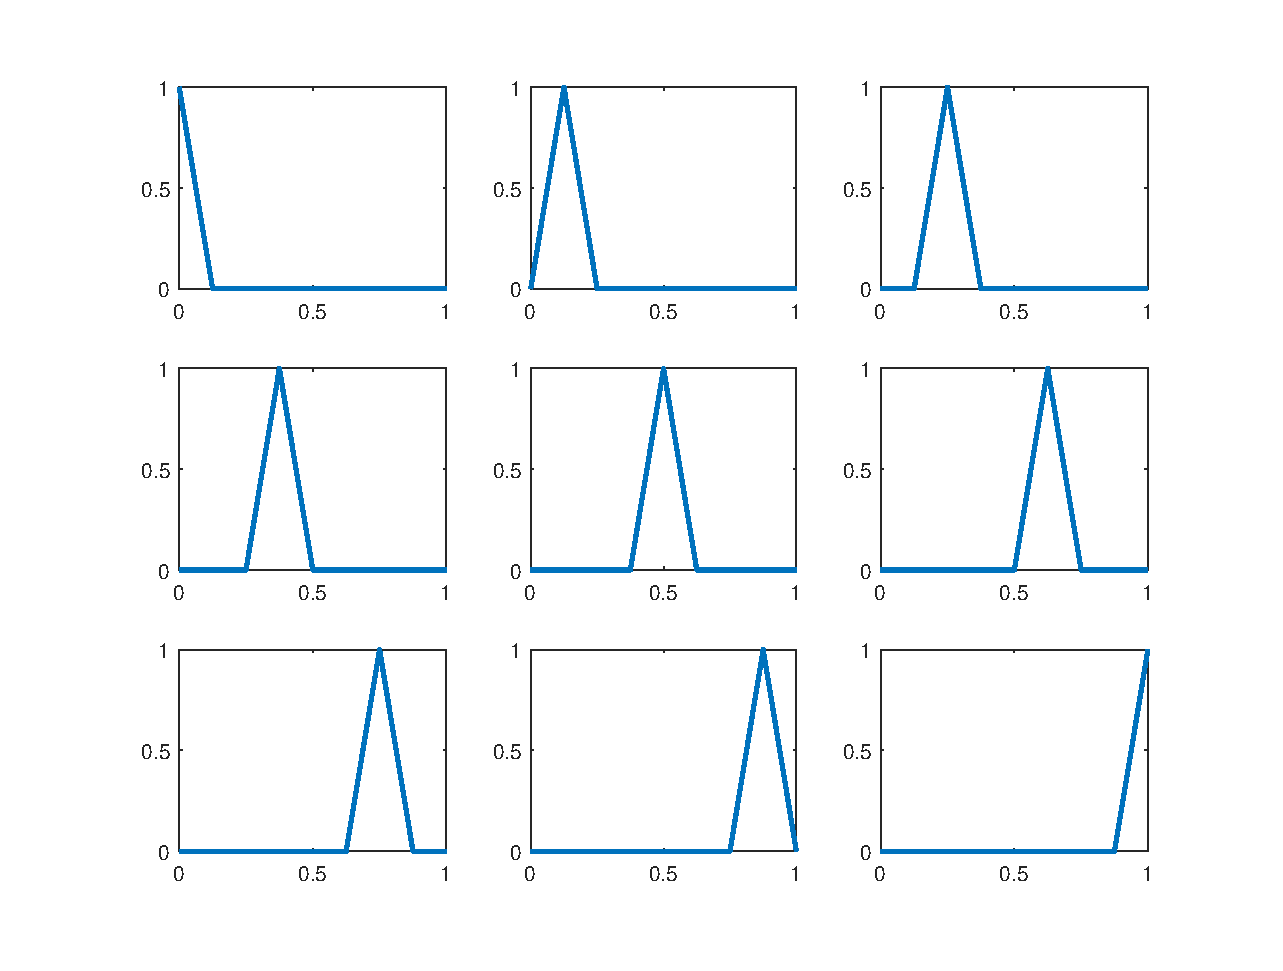
\includegraphics[width = 4in]{linear_spline.eps}
  \end{figure}
\end{frame}

\begin{frame}
\frametitle{Pros and Cons of Linear Splines}
  \begin{itemize}
    \item[--] Pros:
    \begin{itemize}
      \item[1.] Preserves monotonicity and concavity of $f$
      \item[2.] We can exploit information about $f$ clustering more closely together in areas of high curvature in order to increase the accuracy
      \item[3.] Captures binding inequality constraints very well
    \end{itemize}
    \bigskip
    \item[--] Cons:
    \begin{itemize}
      \item[1.] The approximated function is not differentiable at the knots
      \item[2.] The second derivative is 0, and the function is not smooth
    \end{itemize}
  \end{itemize}
\end{frame}

\begin{frame}
\frametitle{Cubic Splines on $\left[0, 1\right]$}
TODO
\end{frame}

\begin{frame}
\frametitle{Pros and Cons of Cubic Splines}
  \begin{itemize}
    \item[--] Pros:
    \begin{itemize}
      \item[1.] Easy to compute: interpolant matrix very sparse, easy to invert
      \item[2.] Smooth approximation
    \end{itemize}
    \bigskip
    \item[--] Cons:
    \begin{itemize}
      \item[1.] It may not be able to handle constraints well
      \item[2.] It does not preserve monotonicity and concavity of $f$
    \end{itemize}
  \end{itemize}
\end{frame}

\section{Example: Income Fluctuation Problem}

\begin{frame}
\frametitle{Income Fluctuation Problem}
  \begin{align*}
    V\left(a,y\right) & =\max_{c,a'} u\left(c\right)+\beta\sum_{y'\in Y}\pi\left(y'|y\right)V\left(a',y'\right)\\
    c+a' & \leqslant Ra+y\\
    a' & \geqslant\underline{a}
  \end{align*}
  \bigskip
  \textcolor{red}{Euler equation} reads
  \[
    u_{c}\left(Ra+y-a'\right)-\beta R\sum_{y'\in Y}\pi\left(y'|y\right)u_{c}\left(Ra'+y'-a''\right)\geqslant0
  \]
  where the strict inequality holds when the constraint is binding
\end{frame}

\begin{frame}
\frametitle{Policy Function Approximation}
  \begin{itemize}
    \item[1.] Choose a set of basis functions $T_{k}$, $k=1,\ldots,n$ and express the policy function as
    \[
      a'=g\left(a,\phi_{y}\right)=\sum_{k=0}^{n}\phi_{y,k}T_{k}\left(a\right)
    \]
    \item[2.] Define the residual function from the Euler equation
    \begin{multline*}
      \mathcal{R}\left(a,\phi_{y}\right)\equiv u_{c}\left(Ra+y-\sum_{k=0}^{n}\phi_{y,k}T_{k}\left(a\right)\right)\\
      -\beta R\sum_{y'\in Y}\pi\left(y'|y\right)u_{c}\left(R\sum_{k=0}^{n}\phi_{y,k}T_{k}\left(a\right)+y'-\sum_{k=0}^{n}\phi_{y',k}T_{k}\left(\sum_{k=0}^{n}\phi_{y,k}T_{k}\left(a\right)\right)\right)
    \end{multline*}
    \item[3.] Using a multidimensional root-finding algorithm to find solutions to
    \[
      \mathcal{R}_{i}\left(a,\phi_{y}\right)=0,i=1,\ldots,n,y\in Y
    \]
  \end{itemize}
\end{frame}

\begin{frame}
\frametitle{Check the Constraint}
  \begin{itemize}
    \item[--] Tell the nonlinear solver that the policy function should be $a'\geqslant\underline{a}$
    \bigskip
    \item[--] In matlab the function \textcolor{blue}{fmincon} allows you to do that
  \end{itemize}
\end{frame}

\end{document}
